% Compile with: lualatex algorithm.tex
\documentclass[11pt,a4paper]{article}

% LuaLaTeX fonts
\usepackage{fontspec}
\usepackage{unicode-math}
\setmainfont{Latin Modern Roman}
\setsansfont{Latin Modern Sans}
\setmonofont{Latin Modern Mono}
\setmathfont{Latin Modern Math}

% Math (amssymb not needed — unicode-math provides all symbols)
\usepackage{amsmath}

% Graphics
\usepackage{graphicx}

% Tables
\usepackage{booktabs}

% Colors (needed for hyperref color mixing)
\usepackage{xcolor}

% Hyperlinks
\usepackage{hyperref}
\hypersetup{
  colorlinks=true,
  linkcolor=blue!70!black,
  citecolor=blue!70!black,
  urlcolor=blue!70!black,
}

% Layout
\usepackage{geometry}
\geometry{margin=2.5cm}

% Paragraph spacing
\usepackage{parskip}

\title{Two-Phase Multi-Point Stochastic Search for Sphere Coloring}
\author{Feodor Pisnitchenko}
\date{}

\begin{document}
\maketitle

\begin{abstract}
We consider the problem of assigning $K$ colors to $N$ points on a sphere so that
the minimum distance between any two same-color points is maximized. The problem
reduces to finding the largest distance threshold $d$ for which the induced conflict
graph is $K$-colorable. We propose a two-phase approach: Phase~1 uses a Conflict
Optimizer to narrow the feasible range quickly, and Phase~2 applies TabuCol with
multi-point stochastic search for fine refinement. A key empirical finding is that
warm-starting TabuCol from a Conflict Optimizer solution traps the search in a
suboptimal basin; fresh randomized greedy initialization overcomes this limitation.
For $N = 64{,}000$ and $K = 1{,}008$, the algorithm achieves a minimum same-color
chord distance of 2714~km (2735~km arc) in 75~minutes on 12~cores.
\end{abstract}

\section{Problem Statement}

Graph coloring is NP-hard. Several practical heuristics exist for large-scale
instances. Hertz and de~Werra \cite{hertz1987} introduced TabuCol, a steepest-descent
tabu search for graph coloring. Moalic and Gondran \cite{moalic2018} developed a
memetic algorithm combining tabu search with crossover. Porumbel et~al.\
\cite{porumbel2010} proposed reactive tabu search with adaptive tenure for
diversification. Schidler and Szeider \cite{schidler2023} introduced SAT-boosted
local search for coloring massive graphs. For geometric intersection graphs,
Crombez et~al.\ \cite{crombez2023} won the CG:SHOP 2022 competition with a conflict
optimization approach. Spatial hashing for efficient neighbor queries
originates from collision detection work by Teschner et~al.\ \cite{teschner2003}.

Given $N$ points on the surface of a sphere (Earth, equatorial radius
$R = 6{,}378.135$~km) arranged in a Fibonacci spiral, and $K$ colors, the goal is to
assign colors to points such that the minimum distance between any two same-colored
points is maximized.

Formally: find the largest chord distance $d^*$ such that there exists a valid
$K$-coloring where no two same-colored points are closer than $d^*$.

This is equivalent to finding the maximum $d$ for which the \textbf{conflict graph}
$G_d = (V, E_d)$ is $K$-colorable, where:
\begin{itemize}
  \item $V = \{0, 1, \ldots, N-1\}$ is the set of points,
  \item $E_d = \{(i, j) : \text{dist}(i, j) < d\}$ is the set of edges connecting
        points closer than $d$.
\end{itemize}

A valid $K$-coloring of $G_d$ assigns each vertex a color from $\{0, 1, \ldots, K-1\}$
such that no edge connects two vertices of the same color. The problem reduces to:
\textbf{find the largest $d$ for which $\chi(G_d) \le K$}, where $\chi(G_d)$ denotes
the chromatic number of $G_d$.

This problem arises in satellite communication systems, where cells represent
coverage zones and colors correspond to frequency channels. Maximizing the minimum
same-color distance reduces co-channel interference.

\textbf{Chord vs.\ arc distance.} Points lie in 3D Euclidean space on the sphere
surface. The chord distance is the straight-line distance through the interior:
$d_{\text{chord}} = \|p_i - p_j\|_2$. The arc (great-circle) distance is the shortest
path along the surface: $d_{\text{arc}} = 2R \arcsin(d_{\text{chord}} / 2R)$. We use
chord distance throughout the algorithm because it requires only a dot product, while arc
distance requires an inverse trigonometric function. The final result is reported in both.

\textbf{Instance parameters.} The main instance studied is $N = 64{,}000$ and
$K = 1{,}008$, giving approximately $\lceil N/K \rceil = 64$ points per color.
Figure~\ref{fig:spiral} shows the Fibonacci spiral distribution on the unit sphere.
Every 8th point is displayed (8{,}000 of 64{,}000), colored by latitude to reveal the
spiral structure that provides near-uniform coverage.

\begin{figure}[htbp]
  \centering
  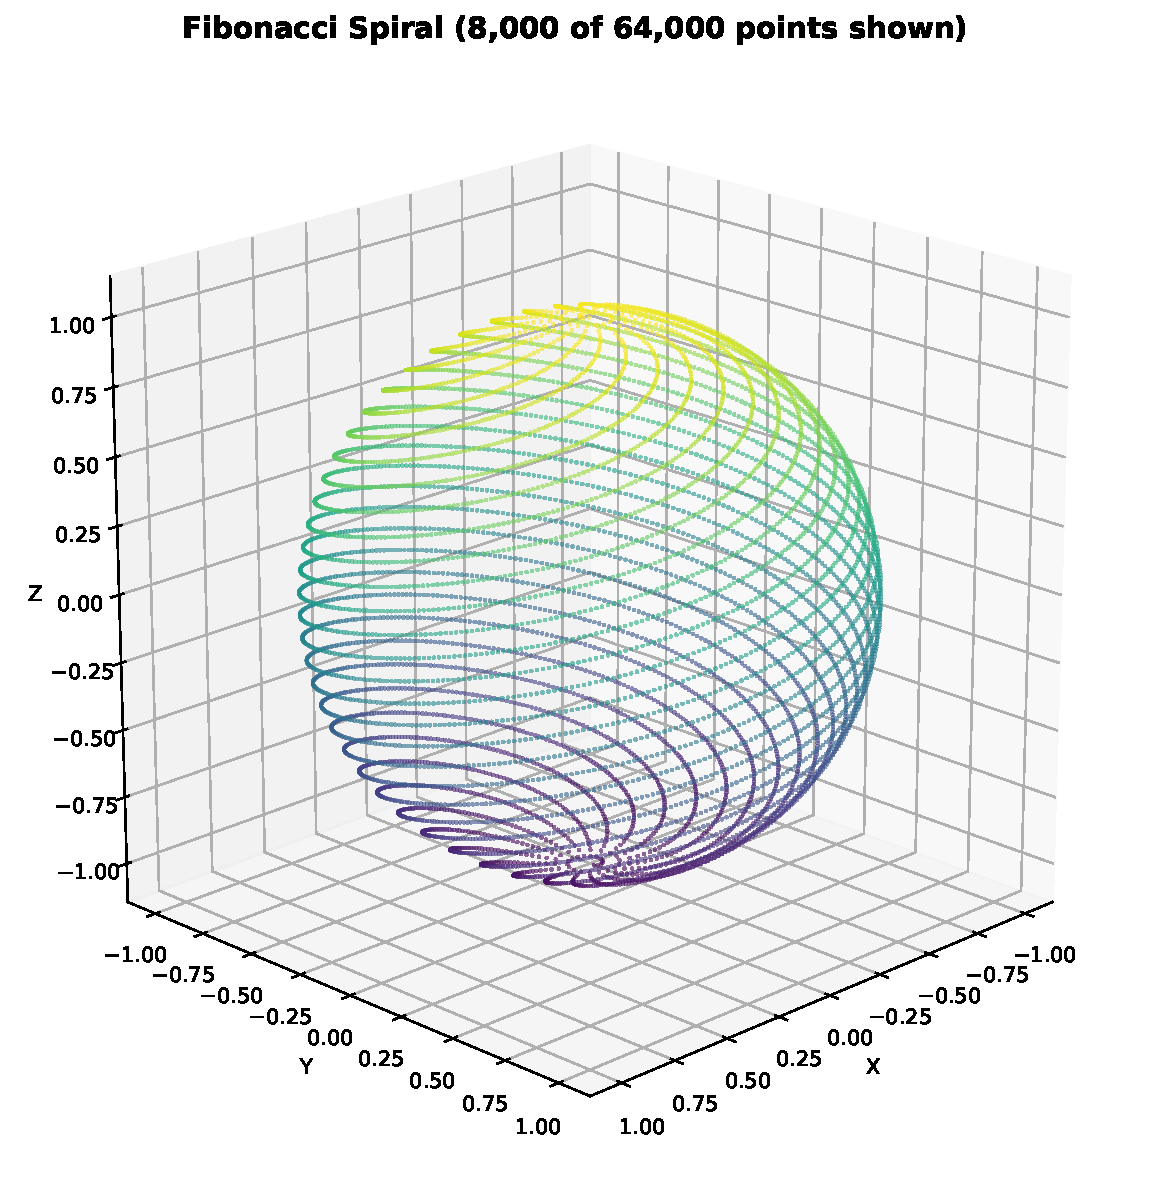
\includegraphics[width=0.6\textwidth]{figures/fig1_fibonacci_spiral.pdf}
  \caption{Fibonacci spiral distribution: 8{,}000 of 64{,}000 points shown
  (every 8th), colored by latitude.}
  \label{fig:spiral}
\end{figure}


\section{Conflict Graph Construction}

For a given chord distance $d$, the conflict graph $G_d$ has an edge between every pair
of points closer than $d$. A naive all-pairs construction costs $O(N^2)$. For
$N = 64{,}000$ this means ${\sim}\, 2 \times 10^9$ distance checks per graph build,
which is too slow when the graph must be rebuilt dozens of times during the search.

\subsection{Spatial Hashing}

We use the spatial hashing technique of Teschner et~al.\ \cite{teschner2003},
originally developed for collision detection. The idea is to partition 3D space
into a grid of cubic cells and map each cell to a hash table bucket. Two points
can be within distance $d$ only if they belong to the same cell or to adjacent
cells. This reduces neighbor search from $O(N^2)$ all-pairs to $O(N \cdot k)$,
where $k$ is the average number of points per cell neighborhood.

Since our points lie on the sphere surface --- a two-dimensional manifold in
three-dimensional space --- we use a cubic grid in Cartesian coordinates.
We set the cell side length to $s = d \times 1.01$ (the 1\% margin avoids
missing pairs due to floating-point rounding). Each point is assigned to the
cell containing its coordinates:
\[
  c_x = \lfloor x / s \rfloor, \quad
  c_y = \lfloor y / s \rfloor, \quad
  c_z = \lfloor z / s \rfloor
\]

Two points can only be neighbors if their cells differ by at most 1 in each
coordinate (the $3 \times 3 \times 3$ neighborhood). Since the points lie on a
surface, most of these 27 cells are empty and skipped immediately. The 3D cubic
grid is simpler than a spherical surface grid, and works efficiently because the
number of non-empty cells is proportional to $4\pi R^2 / s^2$.
The cell key $(c_x, c_y, c_z)$ is hashed using three large primes:
\[
  h = c_x \cdot 73856093 \oplus c_y \cdot 19349663 \oplus c_z \cdot 83492791
\]

\subsection{Two-Pass CSR Construction}

The adjacency is stored in Compressed Sparse Row (CSR) format for cache-friendly
traversal.

\textbf{Pass~1 (count degrees).} Each OpenMP thread maintains a private degree vector.
For each cell, it iterates over the $3 \times 3 \times 3$ neighborhood and checks
pairwise distances. After all cells are processed, thread-local degree vectors are merged
via a critical section.

\textbf{Pass~2 (fill adjacency).} A prefix sum over degrees gives the CSR row pointers.
A sequential pass fills the CSR column indices. The adjacency array uses 32-bit integers
to halve memory: at $d \approx 2700$~km, the graph has ${\sim}\, 92$ million edges, so
the CSR array has ${\sim}\, 184$ million entries (${\sim}\, 736$~MB with 32-bit
vs.\ ${\sim}\, 1.5$~GB with 64-bit).

\textbf{Complexity.} $O(N \cdot \bar{\delta})$ where $\bar{\delta}$ is the average
degree. For $d = 2710$~km: $\bar{\delta} \approx 2900$, so graph construction processes
${\sim}\, 1.9 \times 10^8$ candidate pairs. This is ${\sim}\, 10\times$ faster than the
$O(N^2) \approx 4 \times 10^9$ all-pairs approach.
Figure~\ref{fig:graph} shows how the average vertex degree and edge count grow with the
distance threshold~$d$. At the achieved result $d = 2{,}714$~km, the graph has
approximately 92.7 million edges and average degree ${\sim}\, 2{,}900$. The average
degree of about 2900 means each vertex has many more neighbors than available colors,
making the coloring problem nontrivial at these distances.

\begin{figure}[htbp]
  \centering
  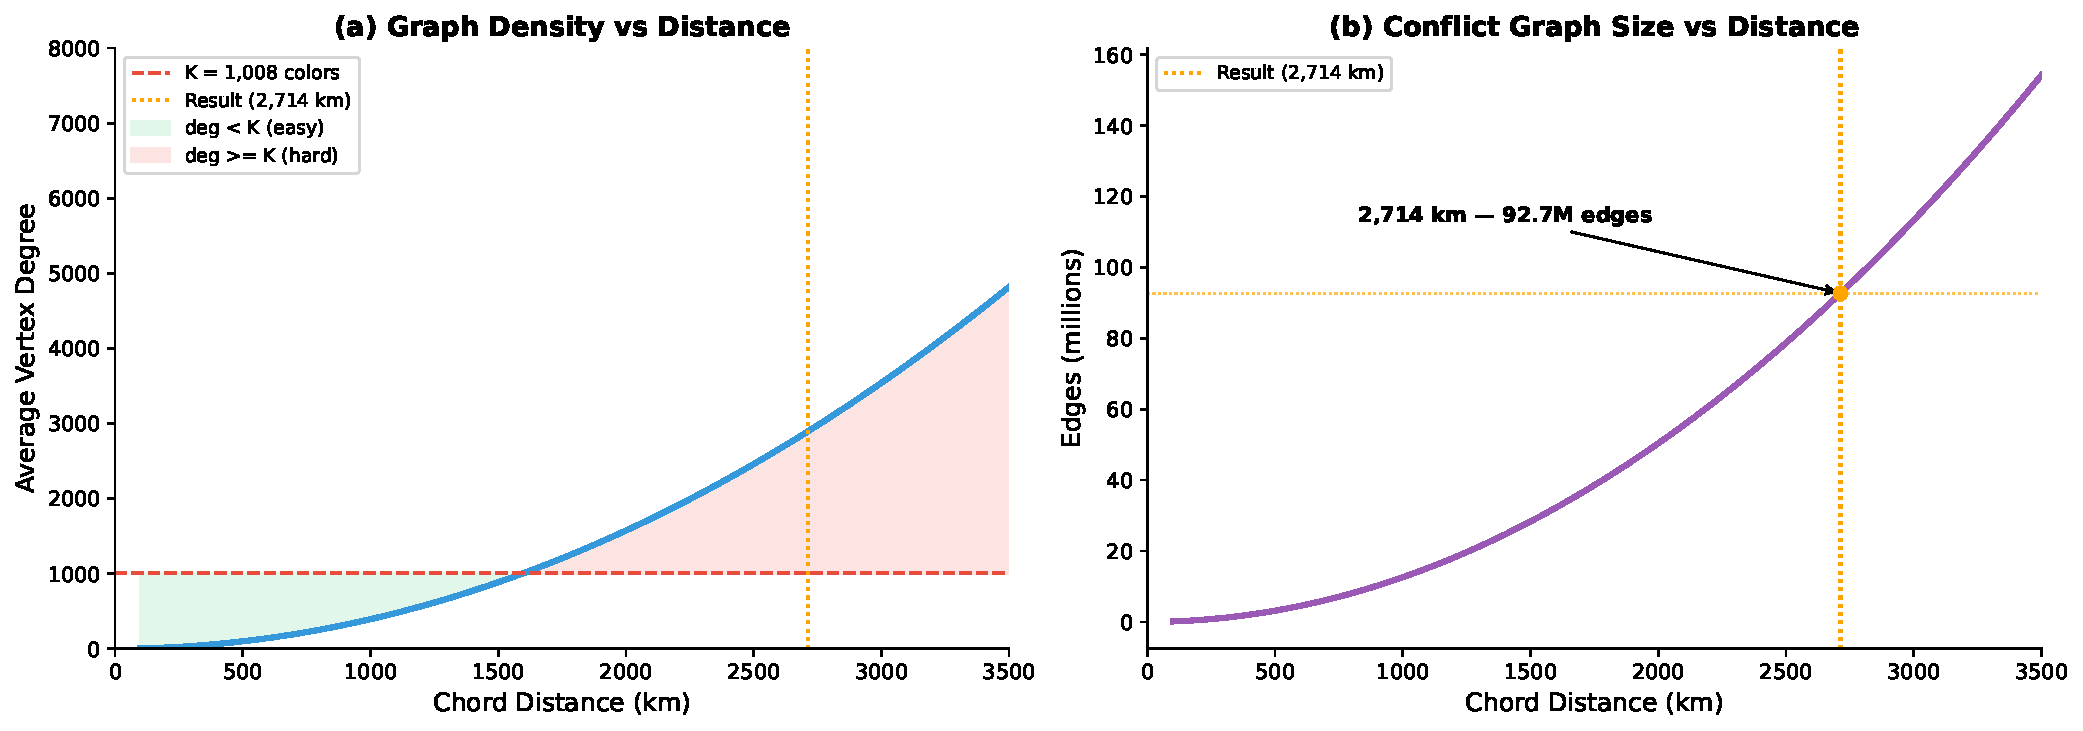
\includegraphics[width=\textwidth]{figures/fig4_graph_properties.pdf}
  \caption{Conflict graph properties as a function of the distance threshold~$d$.
  (a)~Average vertex degree vs.\ distance, with the target $K = 1{,}008$ colors
  shown as a horizontal line. (b)~Total edge count vs.\ distance, with a crosshair
  marking the achieved result at $d = 2{,}714$~km (${\sim}\, 92.7$M edges).}
  \label{fig:graph}
\end{figure}


\section{Heuristic Solvers}

Graph coloring is NP-hard, so we use heuristic solvers that trade optimality guarantees
for practical speed. Two solvers are used: a Conflict Optimizer (CO) for coarse
exploration, and TabuCol for fine refinement. CO runs in seconds per distance point but
reaches a ceiling around $d \approx 2600$~km. TabuCol requires minutes per point but
extends the feasible boundary to $d \approx 2714$~km.

\subsection{Conflict Optimizer (CO)}

Based on the conflict optimization approach of Crombez et~al.\ \cite{crombez2023}.

\textbf{Core idea.} Maintain a partial valid coloring. Conflicting vertices (those
sharing a color with a neighbor) are uncolored and placed in a FIFO queue $S$. Each
iteration:
\begin{enumerate}
  \item Dequeue vertex $v$ from $S$.
  \item For each color $c \in \{0, \ldots, K-1\}$, compute a weighted conflict score:
        the sum of weights $w(u)$ over all colored neighbors $u$ with color $c$.
  \item Assign $v$ the color with the lowest score (after applying Gaussian noise).
  \item Any neighbors of $v$ that now conflict are uncolored and pushed to $S$.
\end{enumerate}

\textbf{Weight function.} $w(u) = 1 + q(u)^p$ where $q(u)$ counts how many times vertex
$u$ has been displaced and $p = 1.2$. Vertices that cycle frequently get higher weights,
steering the algorithm away from colors that cause cascading displacements. The weights
are precomputed in a lookup table to avoid repeated exponentiation.

\textbf{Gaussian noise.} Each non-zero color score is multiplied by a sample from
$\mathcal{N}(1, \sigma)$ with $\sigma = 0.15$. This randomizes tie-breaking and provides
diversification without destroying the weight-based guidance. Scores of zero (no conflict
with that color) are left at zero.

\textbf{Restart logic.} When any vertex's displacement count exceeds a threshold
$q_{\max}$, the search is trapped in a cycle. The algorithm restarts by perturbing the
best coloring found so far: 5\% of vertices are reassigned to random colors. Up to 10
restarts are attempted per run. The threshold scaling
$q_{\max} = 2000 \cdot (75000 / N)^2$, clamped to $\ge 100$, follows \cite{crombez2023}.

\textbf{Complexity per iteration.} $O(\delta(v) + K)$ for vertex $v$ with degree
$\delta(v)$: scanning neighbors costs $O(\delta(v))$, selecting the best color costs
$O(K)$.

CO finds feasible colorings at distances up to $d \lesssim 2600$~km for the main instance
in under 15~minutes. Beyond this threshold, the partial coloring approach cannot resolve
the tightly interlocking conflicts at high edge densities: removing and reinserting one
vertex at a time is insufficient when the color assignment topology itself is suboptimal.


\subsection{TabuCol}

Based on Hertz and de~Werra \cite{hertz1987}, following the standard
steepest-descent formulation.

\textbf{Core idea.} Start from a complete (but possibly invalid) coloring. Each iteration
scans all conflicting vertices across all $K$ colors to find the single best recoloring
move, then applies it.

\textbf{Gamma matrix.} The key data structure is
$\gamma(v, c) = |\{u \in \text{adj}(v) : \text{color}(u) = c\}|$, the count of
neighbors of $v$ with color $c$. This matrix enables $O(1)$ move evaluation:
\[
  \Delta(v, c_{\text{old}} \to c_{\text{new}})
    = \gamma(v, c_{\text{new}}) - \gamma(v, c_{\text{old}})
\]

The total conflict count changes by $\Delta$ when vertex $v$ switches color. After the
move, $\gamma$ is updated for all neighbors of $v$: each neighbor $u$ gets
$\gamma(u, c_{\text{old}})$ decremented and $\gamma(u, c_{\text{new}})$ incremented.
Cost: $O(\delta(v))$.

\textbf{Move selection.} Full scan: for each conflicting vertex $v$ (tracked in a
conflict list) and each color $c \ne \text{color}(v)$, compute $\Delta$. Pick the move
with the smallest $\Delta$ (steepest descent). Ties are broken by smaller vertex index
for deterministic reproducibility.

\textbf{Tabu mechanism.} After moving vertex $v$ from $c_{\text{old}}$ to
$c_{\text{new}}$, the reverse move $(v \to c_{\text{old}})$ is banned for
$T + \text{rand}(0, 10)$ iterations, where $T$ is the current tenure. This prevents
immediate reversal and forces exploration of new regions.

\textbf{Tenure.} Base tenure $T_0 = 0.6\, K$, the standard value from
\cite{hertz1987}. Every 500 iterations without improvement,
$T$ increases by~2 (capped at $K/2$). On a new global best, $T$ resets to $T_0$.

\textbf{Aspiration criterion.} A tabu move is accepted if the resulting total conflicts
would be a new global best. Let $f$ denote the current conflict count and $f^*$ the best
found so far; then the move is accepted when $f + \Delta < f^*$.

\textbf{Stagnation exit.} If no improvement occurs for $20{,}000$ iterations and
$f^* > 5{,}000$, the distance point is abandoned. This saves time when the distance is
far from the feasibility boundary.

\textbf{Conflict list.} Maintained as a dense array with $O(1)$ add/remove via
swap-with-last. A position array enables $O(1)$ lookup of any vertex in the list.

\textbf{Complexity per iteration.} $O(|S| \cdot K)$ where $|S|$ is the number of
conflicting vertices. Near the boundary, $|S|$ is typically a few hundred,
$K = 1{,}008$, giving ${\sim}\, 10^5$ operations per iteration.

TabuCol can solve distances up to ${\sim}\, 2{,}714$~km, roughly 114~km beyond the CO
ceiling. Each iteration is slower than CO at high edge counts due to the full scan over
$|S| \times K$ moves.


\section{Two-Phase Multi-Point Stochastic Search}

The key challenge is that graph coloring feasibility is not monotone in a useful way: a
coloring that works at distance $d$ provides limited guidance for distance $d + \epsilon$,
because the conflict graph changes entirely. Standard binary search requires a reliable
feasibility oracle, but heuristic solvers are stochastic and may fail to find a valid
coloring even when one exists.

\subsection{Overview}

The search proceeds in two phases:
\begin{enumerate}
  \item \textbf{Phase~1 (CO, 15~min):} Multi-point stochastic search with the CO
        solver. Quickly narrows the feasible range from $[0, d_{\max}]$ down to a
        ${\sim}\, 7$~km window around $d \approx 2600$~km.
  \item \textbf{Phase~2 (TabuCol, 60~min):} Multi-point stochastic search with
        TabuCol. Refines the boundary to $d \approx 2714$~km, then binary
        refinement narrows the final gap to $< 0.5$~km.
\end{enumerate}

In practice, warm-starting TabuCol from a CO solution traps it in local
optima. Fresh randomized greedy initialization at high distances works far better (see
Section~\ref{sec:warmstart}).

\subsection{Multi-Point Sampling Strategy}

Each phase operates in rounds. Within a round:
\begin{enumerate}
  \item Divide the current range $[\text{lo}, \text{hi}]$ into $N$ equal subintervals.
  \item Pick a random point within each subinterval (seeded RNG for reproducibility).
  \item For each point (in order from lowest to highest distance):
    \begin{itemize}
      \item Build the conflict graph $G_d$.
      \item Run the heuristic solver.
      \item If feasible: update lo to this distance.
      \item If infeasible and conflicts exceed a cutoff: shrink hi to this distance and
            stop the round (everything above is likely infeasible).
      \item If infeasible but below cutoff: record as the lowest-conflict infeasible
            point.
    \end{itemize}
  \item After the round:
    \begin{itemize}
      \item If any point was feasible: advance lo, keep or increase $N$.
      \item If none feasible: double $N$ for finer sampling in the next round.
      \item Stop when range $< \delta$ or $N$ exceeds the adaptive cap.
    \end{itemize}
\end{enumerate}

The adaptive cap for $N$ is
$\max(N_{\text{init}} \times 8,\; (\text{hi} - \text{lo}) / \delta)$, ensuring
subintervals never become finer than the resolution parameter $\delta$
(\texttt{min\_range}).

\subsection{Phase~1: CO Multi-Point Search}

\begin{itemize}
  \item Initial $N$: 10 subintervals.
  \item Per-point adaptive time budget: 60~seconds for points in the lower 30\% of the
        range, 30~seconds for the middle 30\%, 15~seconds for the upper 40\%. Points
        closer to lo are more likely to be feasible and deserve more solver effort; points
        near hi quickly reveal themselves as infeasible.
  \item Skip threshold ($p_1^{\text{cut}}$): 2000 conflicts. If a point exceeds this, hi
        is shrunk to that distance and the round ends.
  \item Warm-start: CO benefits from warm-start. The best feasible coloring from the
        current round is passed to subsequent points.
  \item Stop condition: range $< 2\delta$ or time budget exhausted.
\end{itemize}

Typical behavior: Phase~1 converges to $[{\sim}\, 2600, {\sim}\, 2607]$ in 5~rounds and
15~minutes.

\subsection{Phase~2: TabuCol Multi-Point Search}

\begin{itemize}
  \item Initial $N$: 5 subintervals.
  \item Per-point time budget: 3~minutes (fixed, not adaptive).
  \item Parallel runs: 12 independent TabuCol instances per distance point, each with a
        different random greedy initialization. The first to reach 0 conflicts signals the
        others to stop.
  \item \textbf{Fresh greedy init} (no warm-start): each TabuCol run starts from a
        randomized greedy coloring computed directly on $G_d$. Run~0 uses ordered greedy
        (deterministic) for reproducibility; runs 1--11 use Fisher--Yates shuffled greedy
        for diversity.
  \item Skip threshold ($p_2^{\text{cut}}$): 500 conflicts. If exceeded, skip remaining
        points in the round (do not shrink hi, because the stochastic nature means nearby
        points may still succeed).
  \item Hard cutoff: $2 \times p_2^{\text{cut}} = 1000$ conflicts. If exceeded, shrink hi
        and end the round.
  \item Density adaptation: if progress within a round is less than 10\% of the remaining
        span, double $N$ for finer sampling.
\end{itemize}

\textbf{Binary refinement.} After the multi-point rounds converge, a binary search
narrows the gap between the best feasible distance and the first infeasible distance. Each
bisection step gets 3~minutes with 12 parallel TabuCol runs. The search stops when the
gap is below $\delta / 4 = 0.5$~km.

Typical behavior: Phase~2 pushes from 2600~km to 2714~km in 6~rounds, then binary
refinement narrows the gap, finishing in 60~minutes.

Figure~\ref{fig:conflicts} shows the conflict count returned by each heuristic at each
tested distance. CO (circles) finds feasible colorings up to ${\sim}\, 2{,}600$~km. TabuCol
(triangles) extends the boundary to ${\sim}\, 2{,}714$~km. The gap between the CO ceiling and
TabuCol's reach illustrates the warm-start trap: CO cannot bridge this region
incrementally, but TabuCol with fresh greedy initialization solves it directly.

\begin{figure}[htbp]
  \centering
  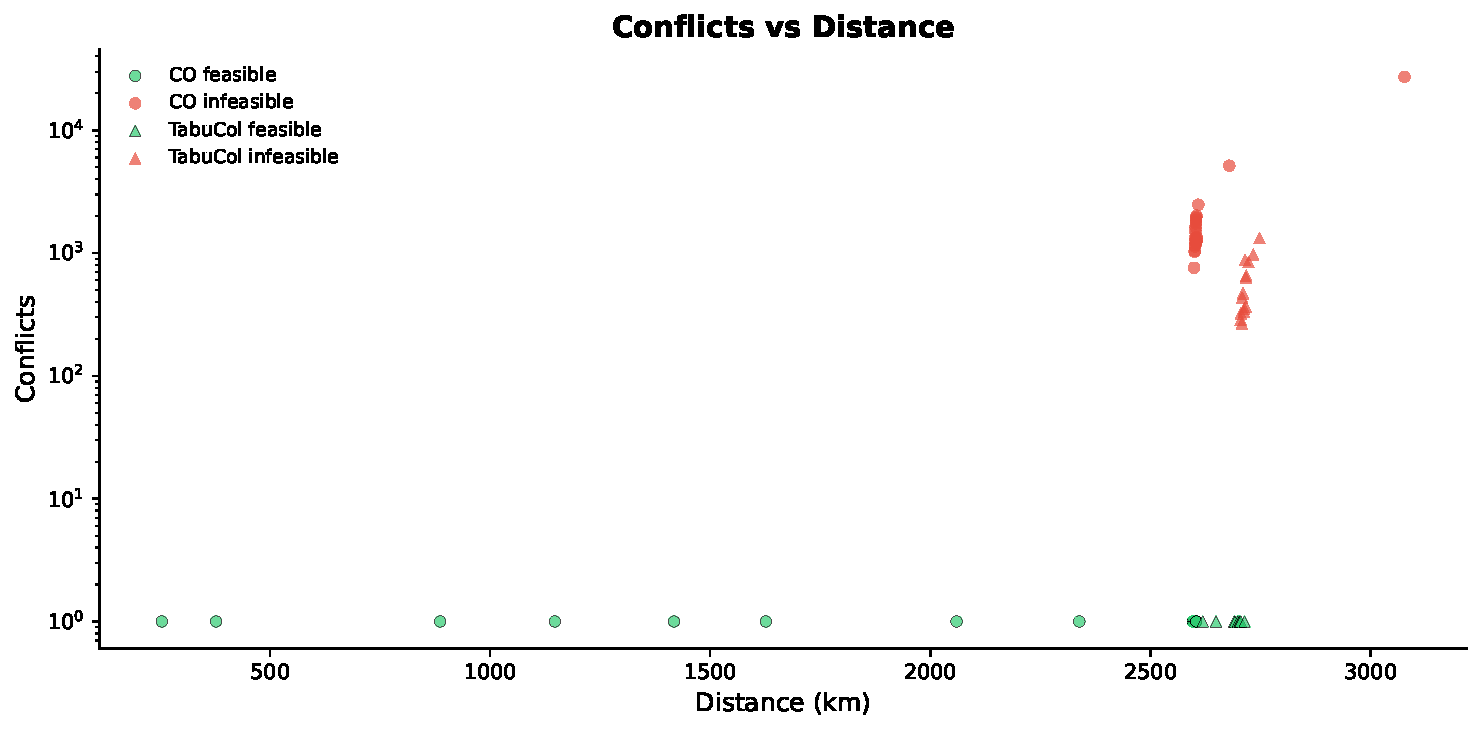
\includegraphics[width=\textwidth]{figures/fig3_conflicts.pdf}
  \caption{Conflict count vs.\ distance for each heuristic run. CO runs (circles) and
  TabuCol runs (triangles) are shown; green markers indicate feasible colorings (zero
  conflicts), red markers indicate infeasible outcomes. CO reaches its ceiling at
  ${\sim}\, 2{,}600$~km, while TabuCol extends feasibility to ${\sim}\, 2{,}714$~km.}
  \label{fig:conflicts}
\end{figure}

\subsection{The Warm-Start Trap}
\label{sec:warmstart}

Consider the following scenario:
\begin{itemize}
  \item CO finds a feasible coloring at $d = 2600$~km.
  \item TabuCol, warm-started from the CO solution, can push to ${\sim}\, 2601$~km. It
        cannot go further.
  \item TabuCol, with a fresh greedy init at $d = 2714$~km (114~km higher):
        \textbf{feasible}.
\end{itemize}

\textbf{Explanation.} CO's coloring has structural bias: it tends to create spatially
clustered color classes (nearby points get similar colors because the
greedy-reassignment process preserves local structure). When the conflict graph grows
denser at higher distances, these clusters create tightly interlocking conflicts that
neither CO nor warm-started TabuCol can untangle, because the overall color assignment
topology is wrong.

A fresh randomized greedy coloring on $G_d$ has no such bias. The random permutation
order produces a more ``random'' color assignment that TabuCol can navigate freely. Even
though it starts with more conflicts, the absence of structural traps allows steepest
descent to find a path to zero.

In combinatorial optimization, a high-quality solution to a related instance can trap
local search in a suboptimal basin of attraction.


\section{Greedy Initialization}

Both CO and TabuCol start from a greedy coloring rather than a random assignment. Two
variants are used:

\subsection{Ordered Greedy}

Process vertices $0, 1, \ldots, N-1$ in index order. For each vertex $v$, count how many
already-colored neighbors have each color, then assign the color with the fewest such
neighbors.

This is deterministic and used for run~0 in each parallel search to ensure
reproducibility.

\subsection{Randomized Greedy}

Generate a random permutation of $\{0, \ldots, N-1\}$ via Fisher--Yates shuffle, then
apply the same min-conflict greedy logic in the shuffled order. A boolean array tracks
which vertices have been processed (since the order is no longer monotone in index).

Each parallel run uses a different seed, producing a different permutation and thus a
different starting coloring. This diversity is essential for the parallel search to
explore different basins.

\textbf{Complexity.} Both variants run in $O(N \cdot \bar{\delta})$: each vertex scans
its neighbors once.


\section{Parameters}

\begin{table}[ht]
\centering
\caption{Algorithm parameters with default values.}
\begin{tabular}{@{}lll@{}}
\toprule
Parameter & Default & Description \\
\midrule
$T_1$ (\texttt{phase1\_min}) & 15~min & Time budget for Phase~1 (CO) \\
$T_2$ (\texttt{phase2\_min}) & 60~min & Time budget for Phase~2 (TabuCol) \\
$I_{\max}$ (\texttt{max\_iters}) & 200,000 & Maximum iterations per single CO or TabuCol run \\
$n_t$ (\texttt{n\_threads}) & 12 & OpenMP thread count (0 = all available CPUs) \\
$d_{\text{lo}}$ (\texttt{lo\_km}) & 0 & Lower bound of search range (0 = start from 0) \\
$d_{\text{hi}}$ (\texttt{hi\_km}) & 0 (auto) & Upper bound of search range. Auto: $4R / \sqrt{\lceil N/K \rceil}$ \\
$p_1^{\text{cut}}$ (\texttt{p1\_cut}) & 2,000 & Phase~1 skip/cut threshold (conflicts) \\
$p_2^{\text{cut}}$ (\texttt{p2\_cut}) & 500 & Phase~2 skip threshold; $2 \times p_2^{\text{cut}}$ is the hard cut \\
$N_1$ (\texttt{p1\_n\_points}) & 10 & Phase~1 initial subintervals per round \\
$N_2$ (\texttt{p2\_n\_points}) & 5 & Phase~2 initial subintervals per round \\
$\delta$ (\texttt{min\_range}) & 2~km & Resolution parameter controlling convergence \\
$s_0$ (\texttt{seed}) & 42 & RNG seed for reproducibility \\
\bottomrule
\end{tabular}
\end{table}

\textbf{Derived thresholds from the resolution parameter $\delta$
(\texttt{min\_range}):}
\begin{itemize}
  \item Phase~1 stops when range $< 2\delta$ (= 4~km).
  \item Phase~2 stops when range $< \delta$ (= 2~km).
  \item Binary refinement stops when gap $< \delta / 4$ (= 0.5~km).
  \item Phase~1 max density: $N_1 \times 8 = 80$ points.
  \item Phase~2 max density:
        $\max(N_2 \times 8,\; \text{range} / \delta)$.
\end{itemize}

\textbf{Automatic range.} The upper bound is derived from a spherical packing bound. With
$K$ colors and $\lceil N/K \rceil$ points per color, the average area per point in a color
class is $4\pi R^2 / N$. The typical spacing between same-color points on a sphere is
approximately $4R / \sqrt{\lceil N/K \rceil}$. For $N = 64{,}000$, $K = 1{,}008$:
$d_{\text{hi}} = 4 \times 6378 / \sqrt{64} \approx 3189$~km.


\section{Results}

Experiments were run on AMD Ryzen AI 9 HX 370 (12 cores used) with 32~GB RAM.

\textbf{Instance:} $N = 64{,}000$ points (Fibonacci spiral), $K = 1{,}008$ colors,
12~threads, seed~42.

\begin{table}[ht]
\centering
\caption{Computational results for $N = 64{,}000$, $K = 1{,}008$.}
\begin{tabular}{@{}ll@{}}
\toprule
Metric & Value \\
\midrule
Best chord distance & 2714~km \\
Best arc distance & 2734.91~km \\
Conflicts & 0 \\
Total time & 75~min 10~sec \\
Phase~1 time & 15~min \\
Phase~2 time & 60~min 10~sec \\
Search steps (lo improvements) & 65 \\
\bottomrule
\end{tabular}
\end{table}

\textbf{Phase~1 (CO) trajectory.} Starting from $[0, 3189]$~km, CO finds feasible
colorings at progressively higher distances: 254, 377, 886, 1147, 1418, 1626, 2060, 2339,
2597, 2600~km. After 5~rounds the range narrows to $[2599.53, 2606.46]$~km. The CO
ceiling is clearly visible: it cannot push past ${\sim}\, 2600$~km regardless of time
invested.

\textbf{Phase~2 (TabuCol) trajectory.} Starting fresh from $[2599.53, 3189.07]$~km,
TabuCol immediately jumps to 2615, then 2645, 2687, 2694, 2701, 2708, and finally
2714~km. The jump from the CO ceiling (2600) to TabuCol's first feasible (2615)
demonstrates the warm-start trap: CO cannot bridge this gap, but fresh greedy + TabuCol
crosses it easily.

\textbf{Binary refinement.} After converging to $[2714, 2720.51]$, binary bisection
steps narrow the boundary. All tested distances above
2714~km are infeasible with 400--1300 remaining conflicts, suggesting 2714~km is
very close to the true feasibility threshold for this seed.

Figure~\ref{fig:convergence} shows the best feasible distance over time. Phase~1 (CO)
rapidly climbs from 0 to ${\sim}\, 2{,}600$~km in 12~minutes (of the 15-minute budget). Phase~2 (TabuCol) then jumps
to ${\sim}\, 2{,}615$~km on its first test point and progressively refines to $2{,}714$~km.

\begin{figure}[htbp]
  \centering
  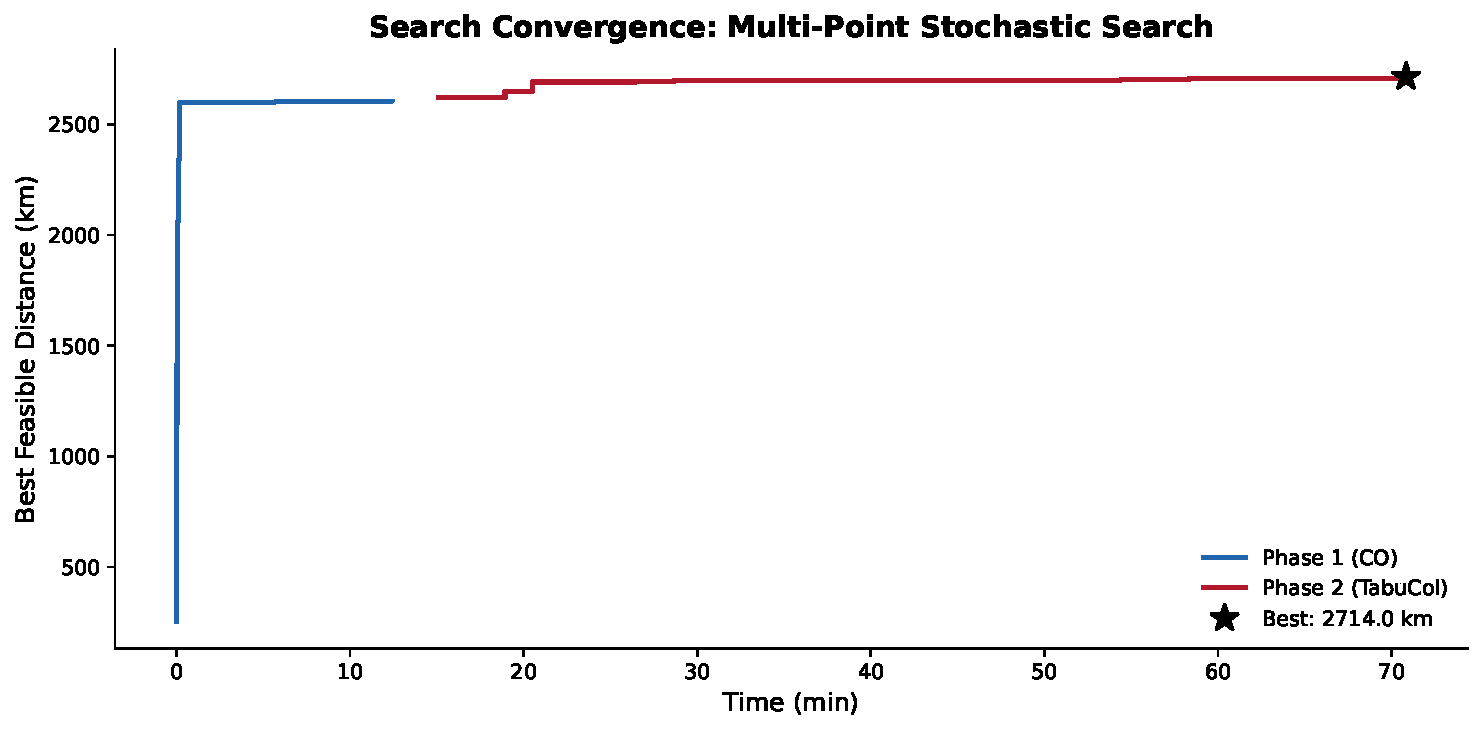
\includegraphics[width=\textwidth]{figures/fig2_convergence.pdf}
  \caption{Best feasible chord distance vs.\ wall-clock time. Phase~1 (CO) climbs
  rapidly from 0 to ${\sim}\, 2{,}600$~km in 12~minutes (of the 15-minute budget). Phase~2 (TabuCol) extends from
  ${\sim}\, 2{,}615$~km to the final $2{,}714$~km over the remaining 60~minutes.
  Each step corresponds to a newly discovered feasible coloring at a higher distance.}
  \label{fig:convergence}
\end{figure}

Figure~\ref{fig:coloring} shows the final coloring on a Mollweide projection. Eight color
classes are highlighted; each contains approximately 64 points spread uniformly across the
globe. The remaining 120 classes are shown in gray. The thin line marks the closest
same-color pair at $2{,}714$~km chord distance.

\begin{figure}[htbp]
  \centering
  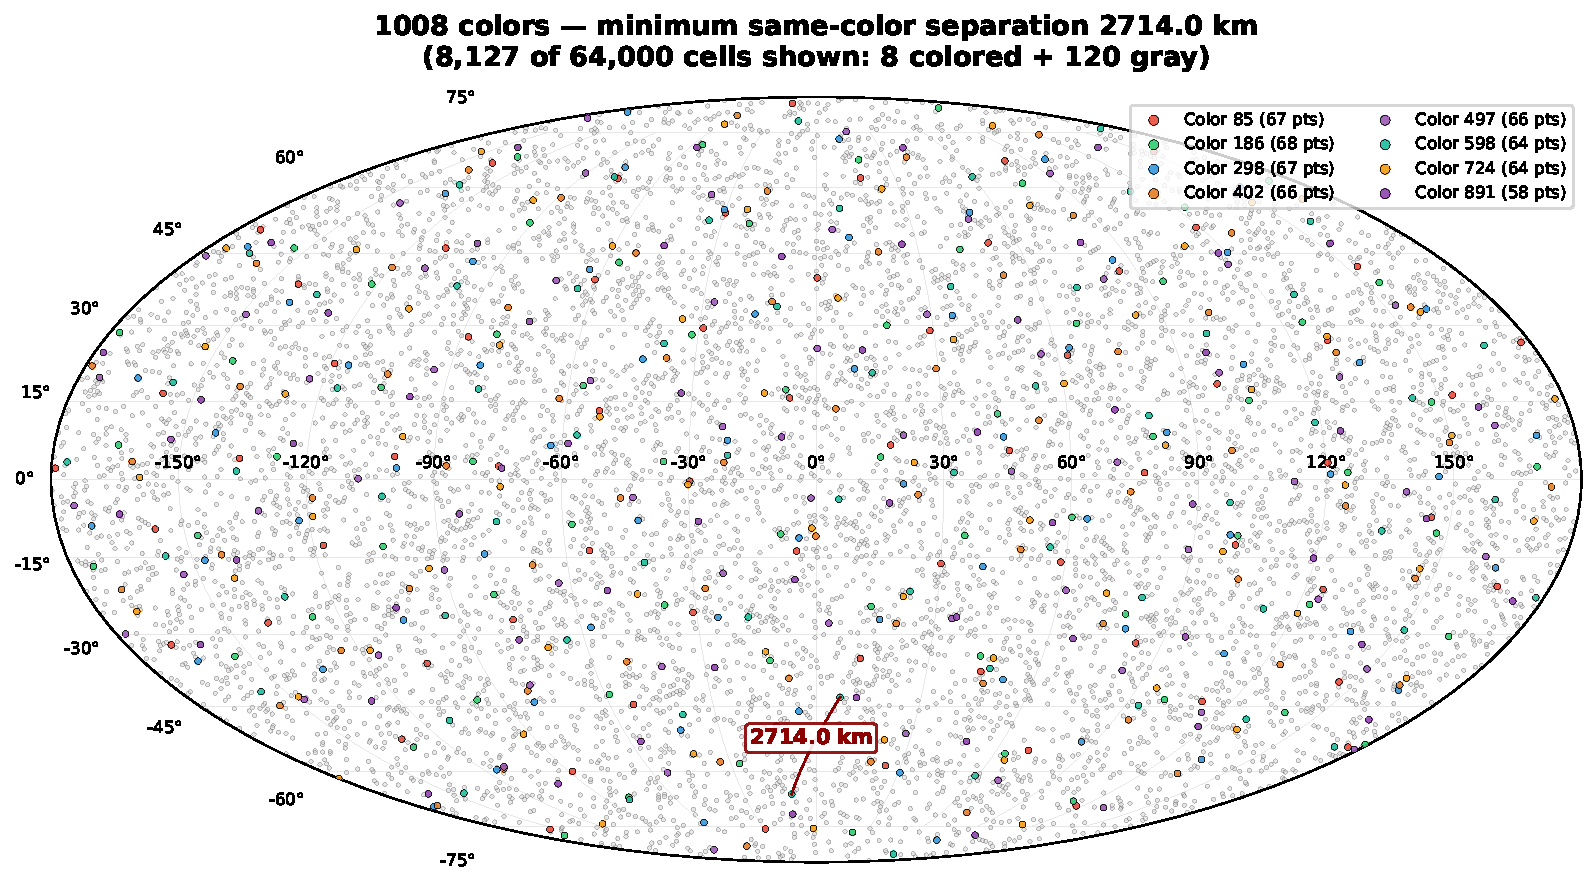
\includegraphics[width=0.6\textwidth]{figures/fig5_coloring.pdf}
  \caption{Mollweide projection of the final $K = 1{,}008$ coloring. Eight
  representative color classes are highlighted to show their near-uniform distribution
  across the sphere. The remaining 120 classes are shown in gray. The annotated line
  connects the closest same-color pair at $2{,}714$~km chord distance.}
  \label{fig:coloring}
\end{figure}

\textbf{Scalability.} The algorithm is parameter-free for different $N$ and $K$: the
search range is computed automatically from the spherical packing bound, thresholds scale
with problem size, and the multi-point structure adapts density based on convergence.


\section{Conclusion}

We presented a two-phase multi-point stochastic search for the sphere coloring problem.
Phase~1 uses a conflict optimizer for fast coarse exploration, and Phase~2 applies TabuCol
with fresh greedy initialization for fine refinement. The key finding is that warm-starting
TabuCol from a conflict optimizer solution traps the search near a suboptimal boundary,
while fresh initialization allows it to reach distances 114~km higher. For $N = 64{,}000$
points and $K = 1{,}008$ colors, the algorithm achieves a minimum same-color chord distance
of 2714~km (2735~km arc) in 75~minutes on 12~cores.

\begin{thebibliography}{9}

\bibitem{crombez2023}
L.~Crombez, G.~da~Fonseca, and Y.~Gerard,
``Conflict Optimization for Binary CSP Applied to Minimum Partition into Plane Subgraphs
and Graph Coloring,''
arXiv preprint arXiv:2303.09632, 2023.

\bibitem{hertz1987}
A.~Hertz and D.~de~Werra,
``Using Tabu Search Techniques for Graph Coloring,''
\textit{Computing}, vol.~39, pp.~345--351, 1987.

\bibitem{moalic2018}
L.~Moalic and A.~Gondran,
``Variations on Memetic Algorithms for Graph Coloring Problems,''
\textit{Journal of Heuristics}, vol.~24, pp.~1--24, 2018.

\bibitem{porumbel2010}
D.~C.~Porumbel, J.~K.~Hao, and P.~Kuntz,
``An Evolutionary Approach with Diversity Guarantee and Well-Informed Grouping
Recombination for Graph Coloring,''
\textit{Computers \& Operations Research}, vol.~37, no.~10, pp.~1822--1832, 2010.

\bibitem{schidler2023}
A.~Schidler and S.~Szeider,
``SAT-Boosted Tabu Search for Coloring Massive Graphs,''
\textit{ACM Journal on Experimental Algorithmics}, vol.~28, Article~1.5, 2023.

\bibitem{teschner2003}
M.~Teschner, B.~Heidelberger, M.~Mueller, D.~Pomeranets, and M.~Gross,
``Optimized Spatial Hashing for Collision Detection of Deformable Objects,''
\textit{Proc.\ VMV}, 2003.

\end{thebibliography}

\end{document}
